

%----------------------------------------------------------------------------------------
%	Corporate Design 2016 Poster
%----------------------------------------------------------------------------------------
%   Last update 05.09.2017 by Reiner Dietz (mailto: reiner.dietz@simtech.uni-stuttgart.de)
%	Last update 17.11.2016 by Mirco Altenbernd.
%
%	For questions or Bug-Reports
%	mailto: mirco.altenbernd@ians.uni-stuttgart.de
%
%----------------------------------------------------------------------------------------
\documentclass[final,hyperref={pdfpagelabels=false},table]{beamer}
%----------------------------------------------------------------------------------------
\usetheme[a0,simtech]{CDP} % Define DIN-size (available: a0, a1, a2, a3, a4) and other options: german, simtech, compactbib
\usepackage[english]{babel}
\usepackage{ragged2e}
\usepackage{blindtext}
\usepackage{amsmath}

%Mathesymbole
\usepackage{amsmath, amsthm, amssymb}
\usepackage{mathrsfs} 

%Schriftarte
\usepackage{times}

%Einbinden von Grafiken
\usepackage{pdfpages}
\usepackage{graphicx}
\usepackage{epstopdf}
%subfigures
\usepackage{subcaption}

%Schriftarten und Symbole
\usepackage{amsfonts}
\usepackage{amssymb}
%\usepackage{bbold}

%Theoreme, Sätze etc.
\usepackage{amsthm}

%Erlaube Seitenumbrüche in \align-Umgebung
\allowdisplaybreaks

%diagonale Linie für Tabelle
\usepackage{diagbox}

%durchstreichen
\usepackage{ulem}

%für autoref
\usepackage{hyperref}

%up Variante griechischer Buchstaben
\usepackage{upgreek}

%ToDo Kommentare
\usepackage{todonotes}

%Algortihms
\usepackage{algorithm}
\usepackage[noend]{algpseudocode}

% a / b fractions 
\usepackage{nicefrac}

%Tikz
\usepackage{tikz}

\usepackage{color}




\graphicspath{{../gfx/}}

%----------------------------------------------------------------------------------------
%   Helpful things and options
%----------------------------------------------------------------------------------------

% table settings and commands for a suiting table style
\usepackage{xparse}
%\DeclareExpandableDocumentCommand{\BodyCell}{m}{\cellcolor{[1,1,1]} #1}
%\DeclareExpandableDocumentCommand{\HeadCell}{m}{\cellcolor{CD01} \color{white} \textbf{#1}}
\DeclareExpandableDocumentCommand{\BodyCell}{m}{\cellcolor{white} #1}
\DeclareExpandableDocumentCommand{\HeadCell}{m}{\cellcolor{white} \color{black} #1}
\makeatletter
\def\arraystretch{1.1}
\arrayrulecolor{white}
\makeatother

% numbered captions
\setbeamertemplate{caption}[numbered]{}

%colors
\definecolor{mittelblau}{RGB}{32,86,174}

%----------------------------------------------------------------------------------------
%   Title - Parameter
%----------------------------------------------------------------------------------------

% The Poster title
\setTitle{High Dimensional Surrogates\\[10pt] 
          with B-Splines for Uncertainty Quantification}

% The Poster subtitle
%\setSubTitle{SimTech}

% Logo subtext (uncomment for Germany-Subtext with english logo)
%\setLogoText{SimTech Cluster of Excellence}
\setLogoText{Cluster of Excellence in Simulation Technology}



% Institute information/address
\setInst{Institut for Parallel and Distributed Systems (IPVS)\\[2pt]
Simulation of Large Systems (SGS)\\[2pt]
Universitätsstr. 38, D-70569 Stuttgart, Germany \\[2pt]
michael.rehme@ipvs.uni-stuttgart.de
}

% Author name
%\setName{\mbox{Michael Rehme}  \\[4pt] Dirk Pflüger}
\setName{\underline{Michael}\\[4pt] \underline{Rehme}\\[4pt]  \ \\[4pt] Dirk \\[4pt] Pflüger}

% uncommand for individual footer layout
 \setFooter{
 \begin{tikzpicture}[remember picture,overlay]
     %left aligned footer-content (image)
     \node[anchor=south west, align=left, yshift=0.01\paperwidth, xshift=0.066\paperwidth] at (current page.south west) {
       
\includegraphics[height=0.035\paperheight]{../gfx/ipvs_logo.png}
       \qquad
       
\includegraphics[height=0.035\paperheight]{../gfx/sgslogo-250x250.png}
       %\includegraphics[height=0.035\paperheight]{mathebanner.pdf}
     };
     %center aligned footer-content (image)
     \node[anchor=south, align=center, yshift=0.01\paperwidth, xshift=0] at (current page.south) {
       % 
\includegraphics[height=0.035\paperheight]{logo_simtech.pdf}
     };
     %center aligned footer-content (text) - yshift may be modified for alignment
     \node[anchor=south, align=center, yshift=0.025\paperwidth, xshift=0] at (current page.south) {
       % {\bfseries\large www.sfbtrr75.de}\\
       % {\bfseries\large www.simtech.uni-stuttgart.de}
     };
     %right aligned footer-content (image)
     \node[anchor=south east, align=right, yshift=0.01\paperwidth, xshift=-0.066\paperwidth] at (current page.south east) {
       
\includegraphics[height=0.035\paperheight]{../gfx/logo_simtech.pdf}
     };
 \end{tikzpicture}
 }

%----------------------------------------------------------------------------------------
%   Content (begin)
%----------------------------------------------------------------------------------------

\begin{document}

\begin{frame}
\centering
\begin{columns}[T]
\begin{column}{\colCWidth}

%----------------------------------------------------------------------------------------
%   Content, left (begin)
%----------------------------------------------------------------------------------------

\justifying
\section{Motivation}
Objective: Construct \textbf{smooth} surrogates for expensive \textbf{high dimensional} models with as few evaluations of these models as possible.
\begin{itemize} 
\item Evaluating the surrogates is much \textbf{faster} than evaluating the original model but provides almost the same results.
\item We use the \textbf{combination technique} and \textbf{Sparse Grids} to overcome the curse of dimensionality.
\end{itemize}

\begin{figure}[h]
\centering
\begin{subfigure}{.47\textwidth}
  \centering
  \tikz[remember picture]\node[inner sep=0pt,outer sep=0pt] (a){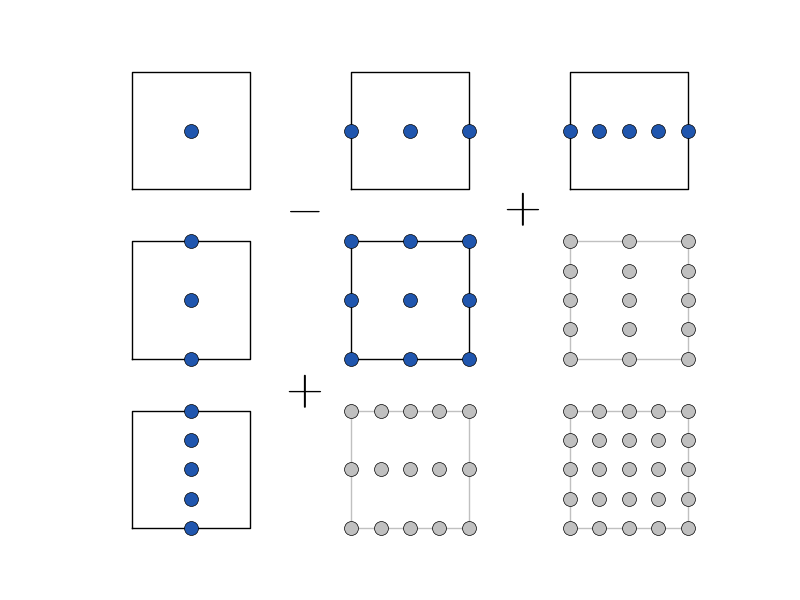
\includegraphics[width=.85\linewidth]{subgrids3.png}};
  \caption*{Subgrid scheme for the combination technique.}
\end{subfigure}%
\begin{subfigure}{.47\textwidth}
  \centering
  \tikz[remember picture]\node[inner sep=0pt,outer sep=0pt] (b){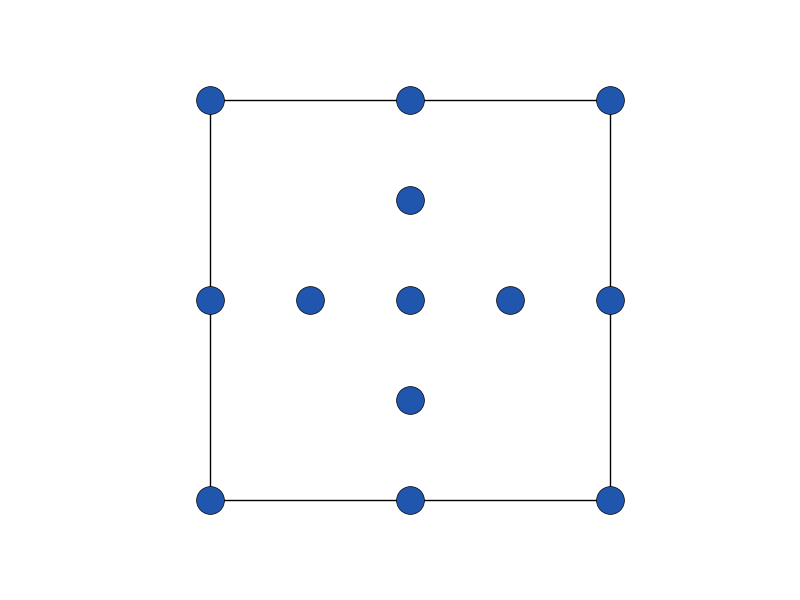
\includegraphics[width=.85\linewidth]{grid3.png}};
  \caption*{Corresponding hierarchical Sparse Grid.}
\end{subfigure}
\tikz[remember picture,overlay]\draw[line width=4pt,-stealth,black] ([xshift=2mm]a.east) -- ([xshift=-2mm]b.west);
\caption{Combination technique and Sparse Grid.}
\end{figure}

\begin{itemize}
\item We use \textbf{not-a-knot B-spline} basis functions to obtain smooth interpolants.
\end{itemize}

\begin{figure}[h]
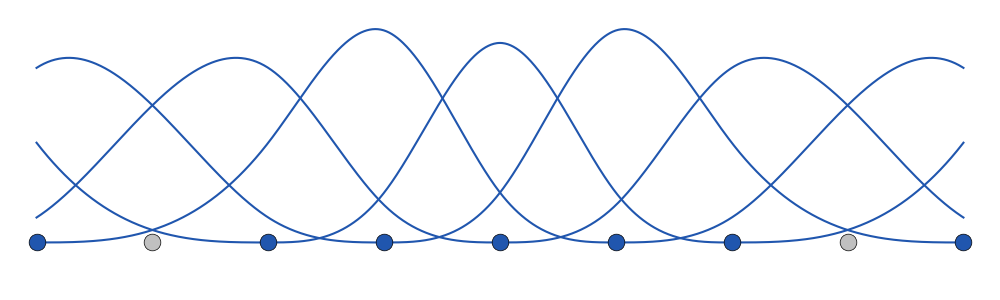
\includegraphics[]{nakBsplineBasis_33.png}
\caption{Not-a-knot B-splines of level 4 and degree 3.}
\end{figure}


\section{Variance Adaptive Refinement}
For the CO$_2$ storage benchmark we want to calculate the \textbf{variance} of the surrogate. Therefore we use the combinations $\Delta_m$ of the variances $v_\ell$ on level $\ell\in\mathbb{N}^d$, as refinement indicators.
\begin{align*}
\Delta_m &= \sum_{\ell \in \mathcal{P}_m} \left( \sum_{ \textbf{0} \leq\alpha \leq \textbf{1}} (-1)^{ \vert \alpha \vert_1}  		v_{\ell - \alpha}\right),\\ \mathcal{P}_m &= \lbrace k \in \mathbb{N}^d: k_i \leq m_i\ \forall i\in \lbrace 1,\dots,d\rbrace\rbrace
\end{align*}

%implemented the following algorithm to create a variance adaptive level structure:
%\begin{itemize}
%\item On each level $\ell$ calculate the variance $v_\ell$.
%\item Calculate $\Delta_m$, the surplus of level $m$, by combining the variances in $\Psi_m$, the set of all predecessors of level $m$.
%\item For all potential new levels $n$ calculate their priority $p_n$ from their direct predecessors $\psi_n \subseteq \Psi_n$.
%\item Add the level with highest priority until the maximum number of points is reached.
%\end{itemize}

\begin{algorithm}[H]
\caption*{Predictive Variance Adaptive Refinement}\label{alg:refine}
\begin{algorithmic}
\Procedure{PVAR}{$M$}\Comment{maximum number of grid points $M$}
\State $\mathcal{L} \leftarrow \lbrace \textbf{0} \rbrace$  
\Comment{initialize level structure $\mathcal{L}$}
\While{$\sum_{\ell \in \mathcal{L} } N(\ell) < M$} 
\Comment{$N(\ell)$ number of grid points of level $\ell$}
\State $\mathcal{F} \leftarrow \lbrace \ell \in \mathbb{N}^d:\ell - e_k \in \mathcal{L}, k\in \lbrace1,\dots,d\rbrace \rbrace$  
\Comment{set of forward neighbors of $\mathcal{L}$}
\For{$\ell \in \mathcal{F} $} 
\State $\mathcal{B}_\ell \leftarrow \lbrace \ell - e_k \in \mathcal{L}:k\in\lbrace1,\dots,d\rbrace,\ell_k>0\rbrace$ \Comment{set of backward neighbors of $\ell$}  
\State{$p_\ell = \nicefrac{1}{\vert \mathcal{B}_\ell \vert} \sum_{m \in \mathcal{B}_\ell} \nicefrac{\vert \Delta_m \vert}{ N(m)}$} \Comment{priorities $p_\ell$}
\State $\mathcal{L} \leftarrow \mathcal{L} \cup argmax_{\ell \in \mathcal{F}} p_\ell$ 
\Comment{add the best candidate to the level structure}
\EndFor
\EndWhile
\State \textbf{return} $\mathcal{L}$
\EndProcedure
\end{algorithmic}
\end{algorithm}


%\begin{itemize}  	
%\item This refinement algorithm can easily be adapted to other objective values than the variance.
%\end{itemize}

\begin{figure}[h]
\centering
%\begin{subfigure}{.47\textwidth}
%\centering
	\begin{tikzpicture}
%square side length
\newcommand*{\Width}{3.5}
%existing levels
\draw [thick](0,0) rectangle (\Width,\Width)node[pos=.5]{$\Delta_{(0,1)}$};
\draw [thick](1.2*\Width,0) rectangle (2.2*\Width,\Width)node[pos=.5]{$\Delta_{(1,1)}$};
\draw [thick](2.4*\Width,1.2*\Width) rectangle (3.4*\Width,2.2*\Width)node[pos=.5]{$\Delta_{(2,0)}$};
\draw [thick](0,1.2*\Width) rectangle (\Width,2.2*\Width);
\draw [thick](1.2*\Width,1.2*\Width) rectangle (2.2*\Width,2.2*\Width);
%potential new levels
\draw [thick, loosely dashed](3.6*\Width, 1.2*\Width) rectangle (4.6*\Width, 2.2*\Width)node[pos=.5]{$p_{(3,0)}$};
\draw [thick, loosely dashed] (2.4*\Width,0) rectangle (3.4*\Width, \Width)node[pos=.5]{$p_{(2,1)}$};
\draw [thick, loosely dashed] (0,-1.2*\Width) rectangle (\Width,-0.2*\Width)node[pos=.5]{$p_{(0,2)}$};
%arrows
\draw[->, line width=2pt] (0.5*\Width, 0.1*\Width) --(0.5*\Width, -0.3*\Width);
\draw[->, line width=2pt] (2.9*\Width, 1.35*\Width) --(2.9*\Width, 0.9*\Width);
\draw[->, line width=2pt] (2.1*\Width, 0.5*\Width) --(2.55*\Width, 0.5*\Width);
\draw[->, line width=2pt] (3.25*\Width, 1.7*\Width) --(3.7*\Width, 1.7*\Width);
\end{tikzpicture}

%\end{subfigure}
%\begin{subfigure}{.47\textwidth}
%\centering
%	\begin{align*}
%		\Delta_m &= \sum_{\ell \in \Psi_m} \left( \sum_{ \textbf{0} \leq\alpha \leq \textbf{1}} (-1)^{ \vert \alpha \vert_1}  		v_{\ell - \alpha}\right)\\
%		\ \\
%		p_n &= \frac{1}{\vert \psi_n\vert} \sum_{m \in \psi_n} \frac{\vert \Delta_m \vert}{ N(m)}\\
%		\ \\
%	\end{align*}
%\end{subfigure}
\caption{Scheme of the variance adaptive refinement.}
\end{figure}

\begin{itemize}
\item We  calculate the final variances on the hierarchical sparse grid corresponding to the adaptively created level structure to reduce the computation time from \textbf{$\mathcal{O}( \vert CT \vert^2)$} to \textbf{$\mathcal{O}(\vert SG \vert^2)$}. \\
\small{$\vert CT \vert$ overall number of points of the combination technique level structure.\\
  	$\vert SG \vert$ number of hierarchical sparse grid points.}
\end{itemize}


%----------------------------------------------------------------------------------------
%   Content, left (end)
%----------------------------------------------------------------------------------------

\end{column}
\begin{column}{\colCWidth}

%----------------------------------------------------------------------------------------
%   Content, right (begin)
%----------------------------------------------------------------------------------------

\justifying
\section{CO$_2$ Storage Benchmark }
As a real world application we examine a benchmark for risk estimation in subterranean CO$_2$ storage. The according model is described in \cite{CO2}.
\subsection{Description}
\begin{figure}
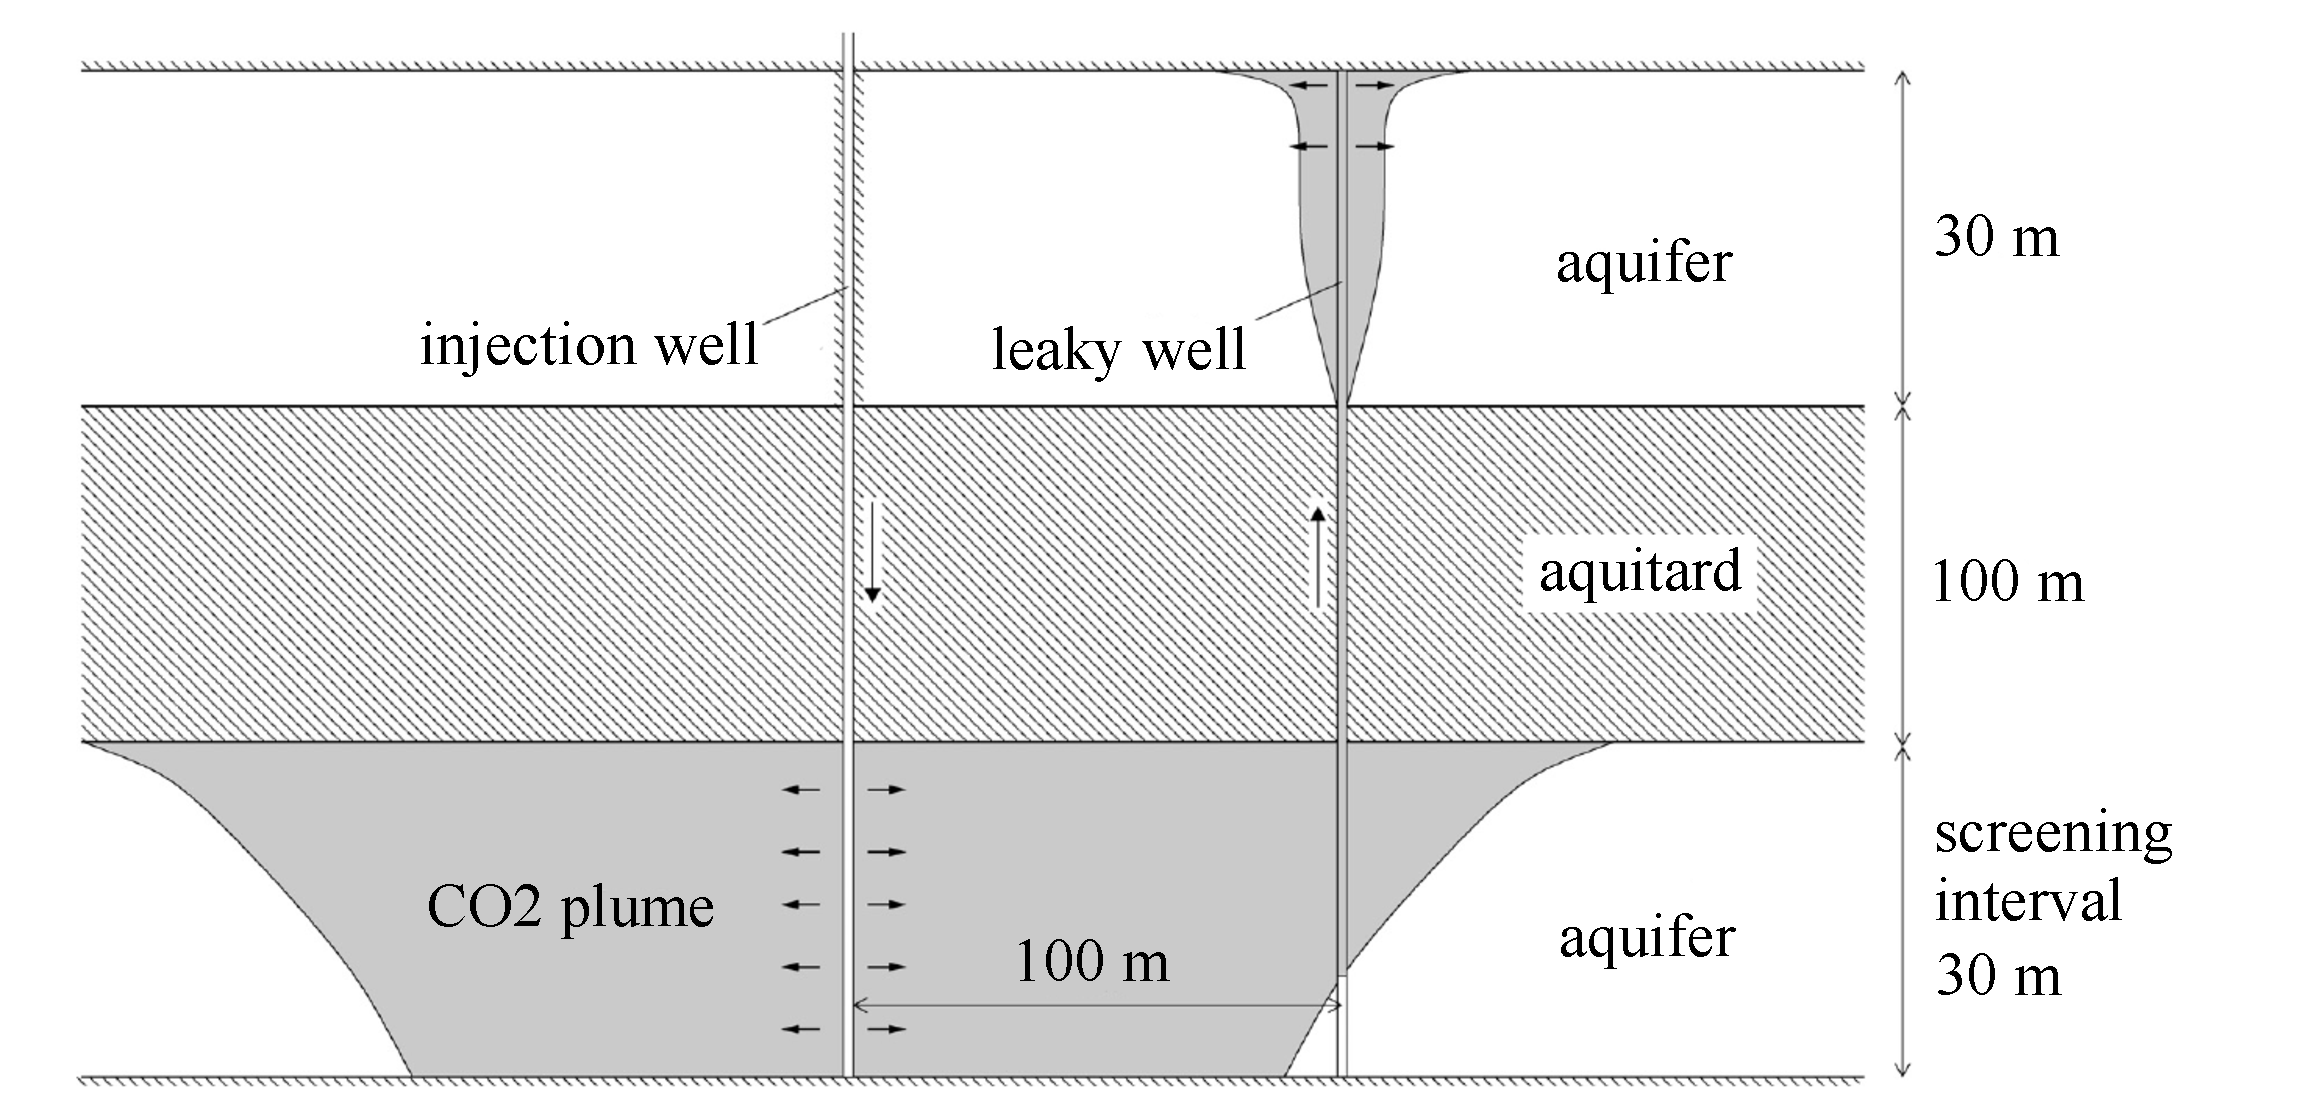
\includegraphics[width=0.8\textwidth]{benchmark.pdf}
\caption{A cross-section of the benchmark example.}
\end{figure}

\begin{itemize}
\item CO$_2$ is injected into a subsurface aquifer, the CO$_2$ starts spreading and reaches a leaky well. Some of the CO$_2$ escapes back to the atmosphere.
\item We are interested in \textbf{expectation value} and \textbf{variance} of the amount of escaping CO$_2$ to decide on the suitability of the CO$_2$ deposit.
\item The underlying multiphase flow processes are highly nonlinear. Therefore solving the models PDEs is very time consuming.
\end{itemize}

\subsection{Numerical Results}

We extended the framework developed for \cite{FF} and created surrogates for the CO$_2$ storage benchmark based on different grid structures and basis functions.

\tikzstyle{mybox}=[draw=mittelblau, fill=white, line width=2.5pt]

\begin{figure}[H]
\begin{minipage}[t]{.3\textwidth}
\begin{tikzpicture}
\node[draw=white, fill=white, line width=2.5pt,rounded corners] {
  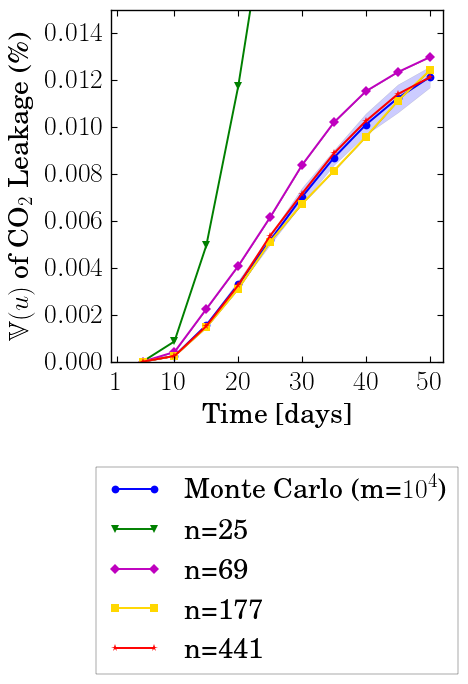
\includegraphics[keepaspectratio=true, width=1.0\columnwidth]{var_analytic_ct_EUB_Re.png}
  };
\end{tikzpicture}
 \caption*{\centering Regular uniform grids with B-splines.}
\end{minipage}
\quad
%\fcolorbox{blue}{white}{
\begin{minipage}[t]{.3\textwidth}
\begin{tikzpicture}
\node[draw=mittelblau, fill=white, line width=2.5pt,rounded corners] {
  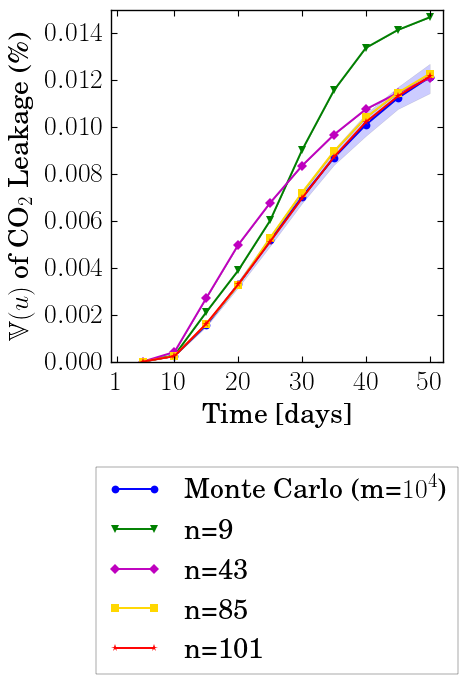
\includegraphics[keepaspectratio=true, width=\columnwidth]{var_analytic_ct_EUB_Va.png}
};
\end{tikzpicture}
\caption*{\centering Adaptive uniform grids with B-splines.}
\end{minipage}
\quad
\begin{minipage}[t]{.3\textwidth}
\begin{tikzpicture}
\node[draw=white, fill=white, line width=2.5pt,rounded corners] {
  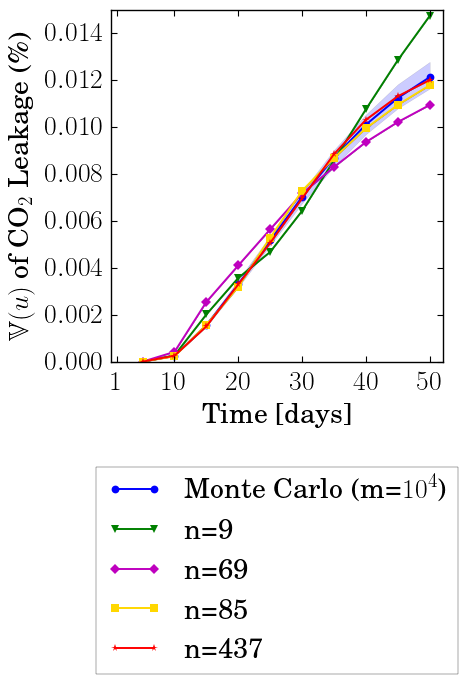
\includegraphics[keepaspectratio=true, width=\columnwidth]{var_analytic_ct_ECC_Va.png}
    };
\end{tikzpicture}
  \caption*{\centering Adaptive Clenshaw-Curtis grids with polynomials.}
\end{minipage}
  \caption{ Variances of the CO$_2$ benchmark problem calculated with different grid types and basis functions. The adaptive uniform grids with B-splines need the smallest number of nodes $n$ for a satisfying approximation of the variance.}
\end{figure}



%\nocite{*} %shows all content within the bibliography file
\section{References}
\normalem %suppresses underlines in bibliography
\bibliography{../literature/references.bib}


%----------------------------------------------------------------------------------------
%   Content, right (end)
%----------------------------------------------------------------------------------------

\end{column}
\end{columns}

\end{frame}
\end{document}

%----------------------------------------------------------------------------------------
%   Content (end)
%----------------------------------------------------------------------------------------
